\chapter{BER理論値を指標とする送信電力制御適用型使用チャネル足切りアルゴリズム
}
本章では,第3章で提案した既存のPPLアルゴリズムについて,研究背景,問題提起をしたのち,これに対する
改善案として3つの内容を検証する.1つ目に伝搬路のSN比が既知であるとしたときのBER理論値を基準とした
獲得固有ベクトル足切りアルゴリズム,2つ目に送信電力分配による理論BER最小化,そして3つ目に,
以上の2つの内容を同時適用した場合を検証する.

\section{研究背景}
第3章では,チャネル推定を行った後に合成チャネル行列を計算して固有値分解する
従来のVCに対して,べき乗法を基本原理とするPPLによる固有ベクトル獲得を提案した.
PPLの最大の特徴は,チャネル推定・合成チャネル行列計算・固有値分解の膨大な演算を,極めて簡単な
非線形処理と無線機間反復処理に置き換えることにある.つまり,伝搬路情報を経由せずに
直接的に固有値・固有ベクトルを求めることができる点に強みがある.
しかし,現在のPPLにおける固有値・固有ベクトルの獲得にかかる無線機間往復数では,実用には十分でないという
問題点がある.固有値問題の性質上,解法には反復解法を用いざるを得ない.PPLではべき乗法を
基本原理としているため,ある程度の反復回数の増加は避けられない.また,VCという方式自体としても
いくつかの課題を有している.その一つに,固有ベクトルに対応する固有値の大きさが,
そのままそのチャネルの利得になっているという特徴上,利得の小さい
チャネルを使用して伝送したデータが,他のチャネルを使用した場合と比較して誤りやすくなるという
問題がある.本章では,上記の二つの問題点に焦点を当て,3つの内容に分けて検証を行う.

\section{検討内容}
ここでは,全部で3つの内容について検討を行う.まず,1つ目としてPPLの課題である無線機間往復数に
対して,一定の通信品質を満たさないチャネルをBER理論値に基づいて足切りすることによる往復数削減
を検証する.2つ目に,VCの課題として挙げた低利得チャネルの誤り率増加減少に対して,送信電力制御
適用によるBER理論値最小化を行う.最後に,1つ目の足切りアルゴリズムに対して,送信電力制御を
組み込んだ場合について検証を行っていく.

\subsection{BER理論値を指標とする使用チャネル足切りアルゴリズム}
ここでは,BER理論値を指標とする使用チャネル足切りアルゴリズムを提案する.
従来のPPLでは,反復処理を行う際,求めたい固有ベクトルの数をあらかじめ
決めたうえで,すべての固有ベクトルが収束するまで反復を行っている.しかし,これは反復回数の面
では無駄が多い.理由として主に以下の3つが挙げられる.1つ目に,べき乗法の特徴として,固有値を大きい順に並べた際に,隣の
固有値との比が大きいほど固有ベクトルの収束が速くなり,逆に小さいほど遅くなるという点が挙げられる.
つまり,求めたい固有ベクトルのうち小さい固有値に対応するものほど,必然的に前の固有値との
比が小さくなるため,獲得までに多くの反復回数を
要することになる.2つ目に,3.5節で説明したように,第2固有ベクトルの獲得では第1固有ベクトルを,
第3固有ベクトルの獲得では第1・第2固有ベクトルを必要とするように,
各固有ベクトルの獲得精度はそれ以前の固有ベクトルの獲得精度の影響を強く受ける.そのため,
後半になるにしたがって,固有ベクトルの獲得精度が低くなり,全体として見たとき拡散符号全体の
直交性が悪化してしまう.3つ目に,固有値が小さい,後半のベクトルほど誤り率が高くなるという
点が挙げられる.VCにおいて,固有値の大きさは各チャネルの利得に対応している.そのため,
固有値の小さいチャネルほど,受信される信号電力が低くなるので,SN比が低下し誤りやすくなるという
特徴がある.上記の理由から,小さい固有値に対応する後半の固有ベクトルを,適切に足切りする
ことができれば,実質的な通信品質を損なわずに不要な反復回数を削減できると考えられる.

図 \ref{figCutoff}に足切りアルゴリズムの概略図,図 \ref{figCutoffFlow}に足切りアルゴリズムのフローチャートを示す.
なお,図 \ref{figCutoff}の固有ベクトル導出に必要な処理は簡略版を示している.
\begin{figure}
    \centering
    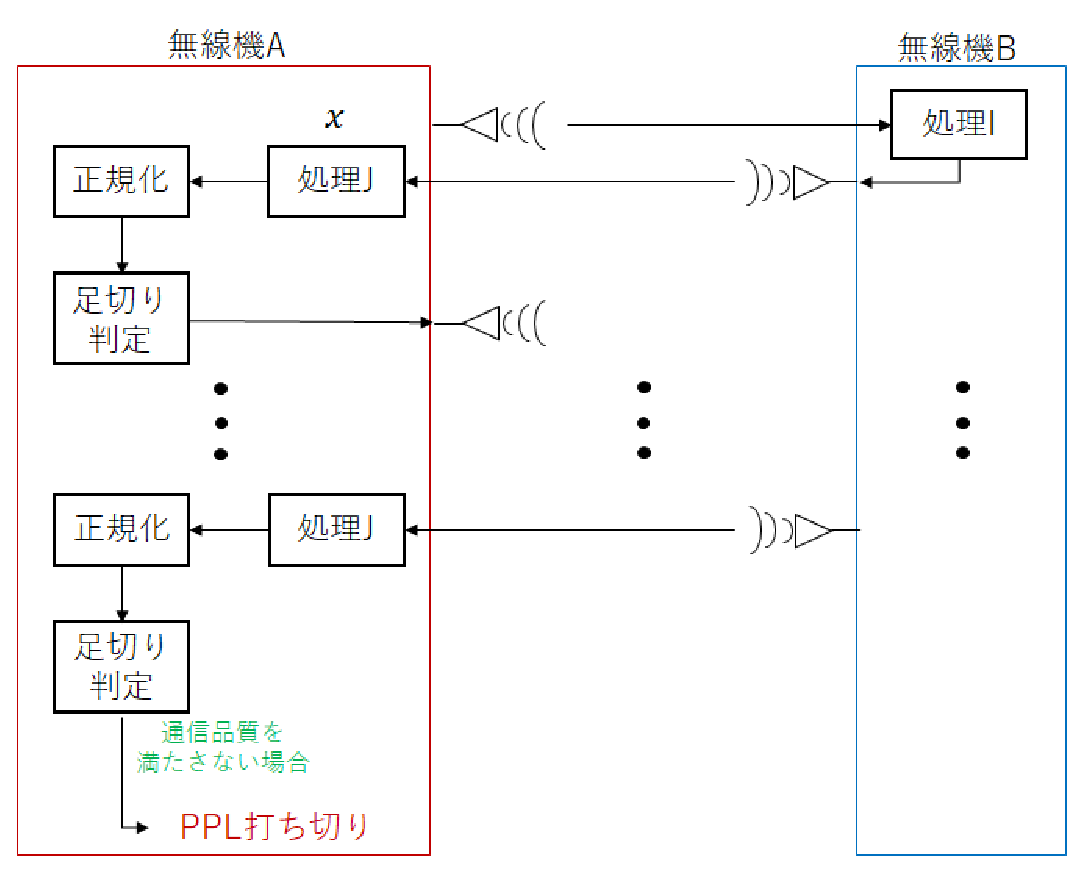
\includegraphics[width=\linewidth]{chapter4/figure/Cutoff.eps}
    \caption{足切りアルゴリズム概略図}
    \label{figCutoff}
\end{figure}
\begin{figure}
    \centering
    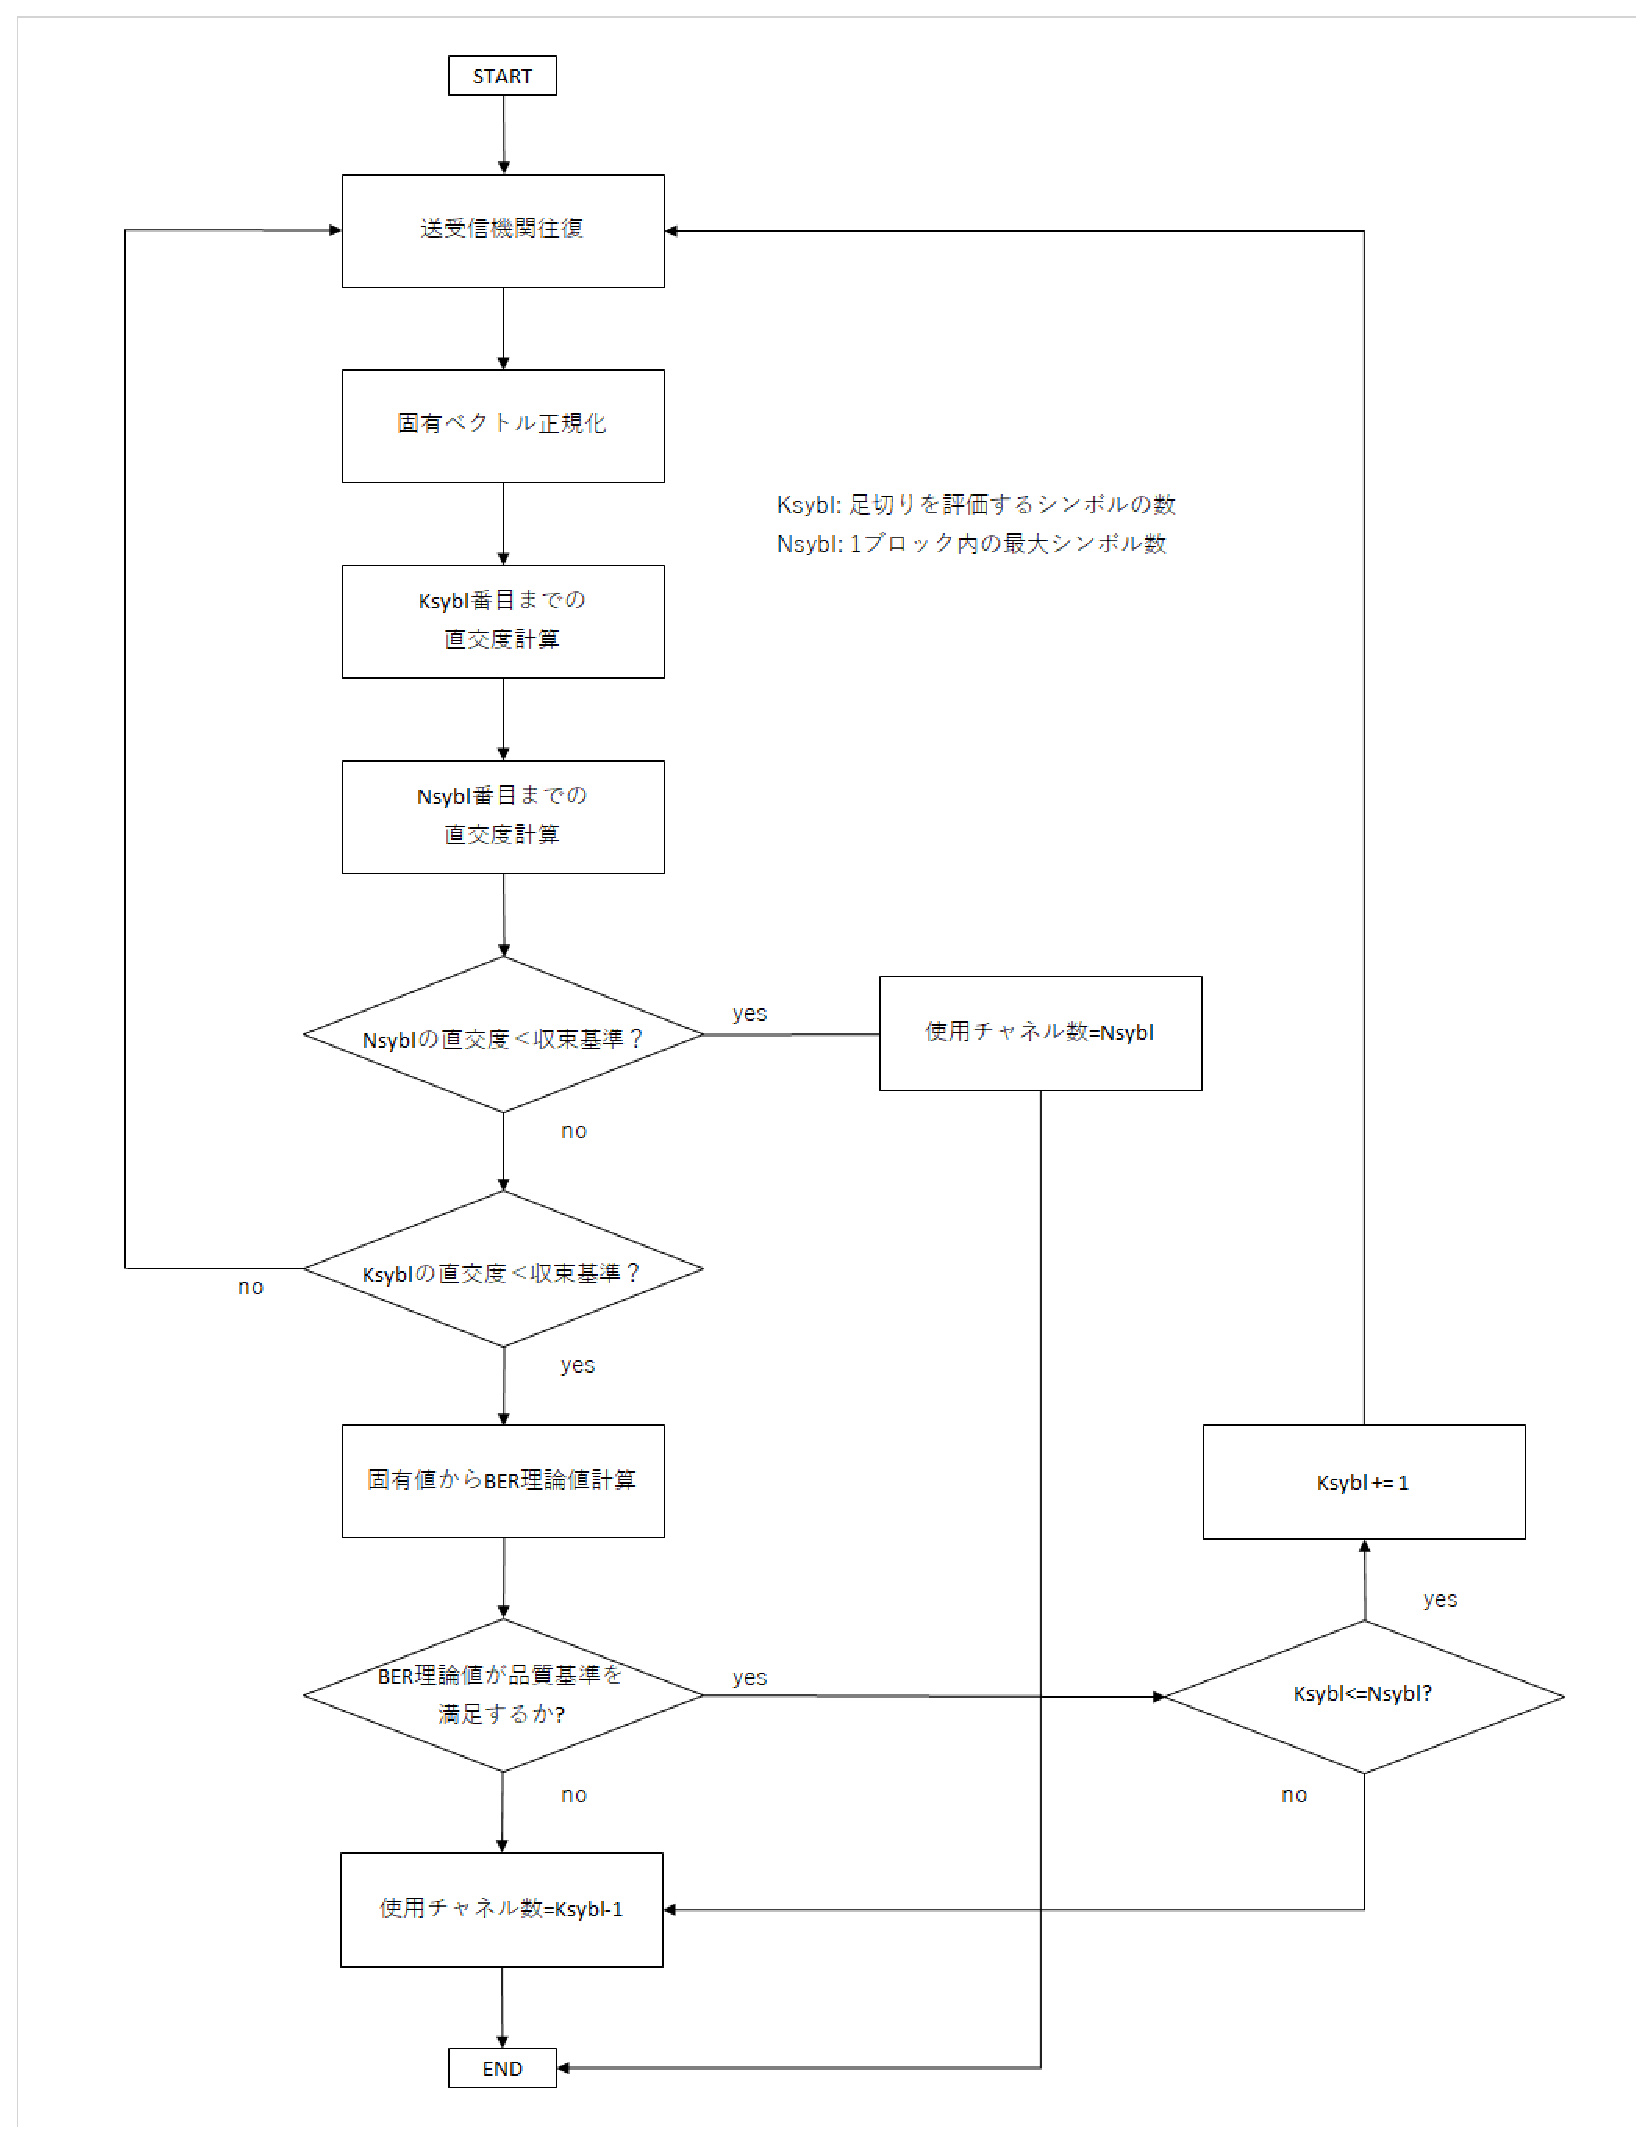
\includegraphics[width=0.95\linewidth]{chapter4/figure/CutoffFlow.eps}
    \caption{足切りアルゴリズムフローチャート}
    \label{figCutoffFlow}
\end{figure}
図 \ref{figCutoff}のNsyblは最大獲得固有ベクトル数,Ksyblは足切り評価を行う固有ベクトル数に
なっている.また,固有ベクトルの収束判定基準に使用する直交度は以下のように定義するものとする.\\
\vspace{5mm}
(例) \quad 固有ベクトルが$\bm{u_1,u_2,u_3}$の3つの場合を考える.
\begin{equation}
    直交度 = \left|\bm{u_1^Hu_2}\right|+\left|\bm{u_1^Hu_3}\right|+\left|\bm{u_2^Hu_3}\right|
\end{equation}

具体的にどのように足切り判定が行われるか図 \ref{figCutoffFlow}をもとに説明する.
まず,任意ベクトル$\bm{x}$の送受信機関往復を行った後,正規化を行いKsybl番目までの
直交度を計算する.Ksyblの初期値は$Ksybl=2$とする.その後,Nsybl番目まで(全固有ベクトル)
の直交度を計算する.これは,Ksybl番目までよりNsybl番目の直交度が速く収束した場合に,
優先してNsybl番目まで使用した際の通信品質を評価するためである.直交度の定義的に,
十分収束したと判断するための収束基準は,評価する固有ベクトルの数が少ないほど厳しくなる.
そのため,Nsybl番目まで見たときのほうが先に収束する場合が稀に存在するので,以上の処理を
挿入している.Nsyblまでの直交度が十分な場合,$使用チャネル数=Nsybl$として,
図中のEndに飛ぶ.直交度が不十分な場合,Ksyblまでの直交度評価に移る.
Ksyblまでの直交度が不十分な場合は,無線機間往復に戻る.直交度が十分な場合は,
固有値からBER理論値を計算し,当該理論値があらかじめ設定した品質基準を満足するか判定にかける.
品質を満たさない場合は,Ksybl番目のチャネル品質が悪いということになるので,$使用チャネル数=Ksybl-1$
として,Endに移行する.品質判定において,品質基準を満足する場合は$Ksybl \leq Nsybl$の時は
Ksyblを1増やして無線機間往復に戻る.$Ksybl>Nsybl$の時はすべての固有ベクトルが収束し,
かつすべてのチャネルを使用しても通信品質を満足するということなので,足切りを終了する.

\subsection{送信電力制御を用いたBER理論値最小化}
\subsection{送信電力制御適用時の使用チャネル足切りアルゴリズム}

\section{検証}
\subsection{BER理論値を指標とする使用チャネル足切りアルゴリズム}
\subsubsection{シミュレーション諸元}
\subsubsection{シミュレーション結果}
\subsection{送信電力制御を用いたBER理論値最小化}
\subsubsection{シミュレーション諸元}
\subsubsection{シミュレーション結果}
\subsection{送信電力制御適用時の使用チャネル足切りアルゴリズム}
\subsubsection{シミュレーション諸元}
\subsubsection{シミュレーション結果}
